\documentclass[../../main.tex]{subfiles}
\graphicspath{{../../image/}{../../figure/}}
\begin{document}

\section{通用图网络}\label{section:ch13-通用图网络}

迄今为止我们所考虑的图网络有许多变体和扩展。这里我们概述一些关键概念以及一些实践考虑。

\subsection{图注意力网络}\label{subsection:ch13-图注意力网络}

注意力机制在作为~Transformer~架构的基础时展现出强大的能力（参见~12.1~节）。在图神经网络中，注意力机制可以用于构建一种能够整合来自邻居节点信息的聚合函数。在这种机制中，传入的消息会根据注意力系数 $A_{nm}$ 加权，从而得到
\begin{align}
\bm{z}_n^{(l)}=\operatorname{Aggregate}\!\left(\{\bm{h}_m^{(l)}:m\in\mathcal{N}(n)\}\right)=\sum_{m\in\mathcal{N}(n)}A_{nm}\,\bm{h}_m^{(l)}
\label{align:ch13-attn-agg}
\end{align}
其中，注意力系数满足
\begin{align}
A_{nm}&\geq 0
\label{align:ch13-attn-nonneg}\\
\sum_{m\in\mathcal{N}(n)}A_{nm}&=1.
\label{align:ch13-attn-norm}
\end{align}

这种网络称为图注意力网络（graph attention network）（Veličković et al., 2017），它可以捕获一种归纳偏置，该归纳偏置表明在确定最佳更新的过程中，某些相邻节点比其他节点更重要，而这种重要性取决于数据本身。

构建注意力系数的方法有很多种，但通常都会使用~softmax~函数。例如，我们可以使用双线性形式
\begin{align}
A_{nm}=\frac{\exp\!\left(\bm{h}_n^{\mathsf T}\bm{W}\bm{h}_m\right)}{\sum_{m'\in\mathcal{N}(n)}\exp\!\left(\bm{h}_n^{\mathsf T}\bm{W}\bm{h}_{m'}\right)}
\label{align:ch13-attn-bilinear}
\end{align}
其中 $\bm{W}$ 是一个 $D\times D$ 的可学习参数矩阵。一种更通用的选择是使用神经网络组合边的两个端点的节点的嵌入向量：
\begin{align}
A_{nm}=\frac{\exp\!\left\{\operatorname{MLP}(\bm{h}_n,\bm{h}_m)\right\}}{\sum_{m'\in\mathcal{N}(n)}\exp\!\left\{\operatorname{MLP}(\bm{h}_n,\bm{h}_{m'})\right\}}
\label{align:ch13-attn-mlp}
\end{align}
其中~MLP~具有单个的连续输出变量，并且当输入向量交换时，这个输出变量的值不变。只要~MLP~在网络中的所有节点之间是共享的（见习题~13.8），这个聚合函数就会在节点重新排序下保持等变性。

图注意力网络可以通过引入多头注意力机制来进行扩展，在这个机制中，我们可以定义 $H$ 组不同的注意力权重 $A_{nm}^{(h)}$，$h=1,\cdots,H$。每个注意力头都使用上面描述的机制之一进行计算，并且具有自己的独立参数（参见~12.1.6~节）。然后在聚合步骤中使用拼接和线性投影将它们组合起来。需要注意的是，对于全连接网络，多头图注意力网络就变成标准的~Transformer~编码器（见习题~13.9）。

\subsection{边嵌入}\label{subsection:ch13-边嵌入}

前面讨论的图神经网络使用的嵌入向量都与节点相关联。我们已经看到一些网络也具有与边相关联的数据。即使不存在与边相关联的观测值，我们也仍然可以维护和更新基于边的隐藏变量，这些变量可以为图神经网络学习的内部表示做出贡献。

除了由 $\bm{h}_n^{(l)}$ 给出的节点嵌入，我们还引入了边嵌入 $\bm{e}_{nm}^{(l)}$。然后我们可以使用以下形式定义一般的消息传递方程：
\begin{align}
\bm{e}_{nm}^{(l+1)}&=\operatorname{Update}_{\mathrm{edge}}\!\left(\bm{e}_{nm}^{(l)},\bm{h}_n^{(l)},\bm{h}_m^{(l)}\right)
\label{align:ch13-edge-update}\\
\bm{z}_n^{(l+1)}&=\operatorname{Aggregate}_{\mathrm{node}}\!\left(\{\bm{e}_{nm}^{(l+1)}:m\in\mathcal{N}(n)\}\right)
\label{align:ch13-edge-agg}\\
\bm{h}_n^{(l+1)}&=\operatorname{Update}_{\mathrm{node}}\!\left(\bm{h}_n^{(l)},\bm{z}_n^{(l+1)}\right).
\label{align:ch13-edge-node-update}
\end{align}

最终层学习到的边嵌入 $\bm{e}_{nm}^{(l)}$ 可以直接用来预测与边相关的内容。

\subsection{图嵌入}\label{subsection:ch13-图嵌入}

除了节点嵌入和边嵌入，我们还可以维护和更新与整个图相关的嵌入向量 $\bm{g}^{(l)}$。将所有这些方面结合在一起，我们便能够为图结构化应用定义更通用的一组消息传递函数，以及更丰富的学习表示集合。具体来说，我们可以定义如下消息传递方程（Battaglia et al., 2018）：
\begin{align}
\bm{e}_{nm}^{(l+1)}&=\operatorname{Update}_{\mathrm{edge}}\!\left(\bm{e}_{nm}^{(l)},\bm{h}_n^{(l)},\bm{h}_m^{(l)},\bm{g}^{(l)}\right)
\label{align:ch13-edge-update-g}\\
\bm{z}_n^{(l+1)}&=\operatorname{Aggregate}_{\mathrm{node}}\!\left(\{\bm{e}_{nm}^{(l+1)}:m\in\mathcal{N}(n)\}\right)
\label{align:ch13-edge-agg-g}\\
\bm{h}_n^{(l+1)}&=\operatorname{Update}_{\mathrm{node}}\!\left(\bm{h}_n^{(l)},\bm{z}_n^{(l+1)},\bm{g}^{(l)}\right)
\label{align:ch13-node-update-g}\\
\bm{g}^{(l+1)}&=\operatorname{Update}_{\mathrm{graph}}\!\left(\bm{g}^{(l)},\{\bm{h}_n^{(l+1)}:n\in\mathcal{V}\},\{\bm{e}_{nm}^{(l+1)}:(n,m)\in\mathcal{E}\}\right).
\label{align:ch13-graph-update}
\end{align}

这些消息传递方程首先更新边嵌入向量 $\bm{e}_{nm}^{(l+1)}$，该操作是基于边嵌入向量的先前状态，每条边连接的节点的嵌入向量，以及图级嵌入向量 $\bm{g}^{(l)}$ 进行的，参见式\eqref{align:ch13-edge-update-g}。然后将这些更新的边嵌入向量在连接到每个节点的每条边上进行聚合，参见式\eqref{align:ch13-edge-agg-g}。接下来转而利用当前节点的嵌入向量和图级嵌入向量更新节点嵌入向量 $\bm{h}_n^{(l+1)}$，参见式\eqref{align:ch13-node-update-g}。最后基于图中所有节点和所有边的信息，以及从前一层获得的图级嵌入向量，更新当前层的图级嵌入向量。\cref{fig:ch13-msg-update}演示了上述过程，算法~13.2~对图消息传递更新做了总结。

\begin{figure}[htbp]
\centering
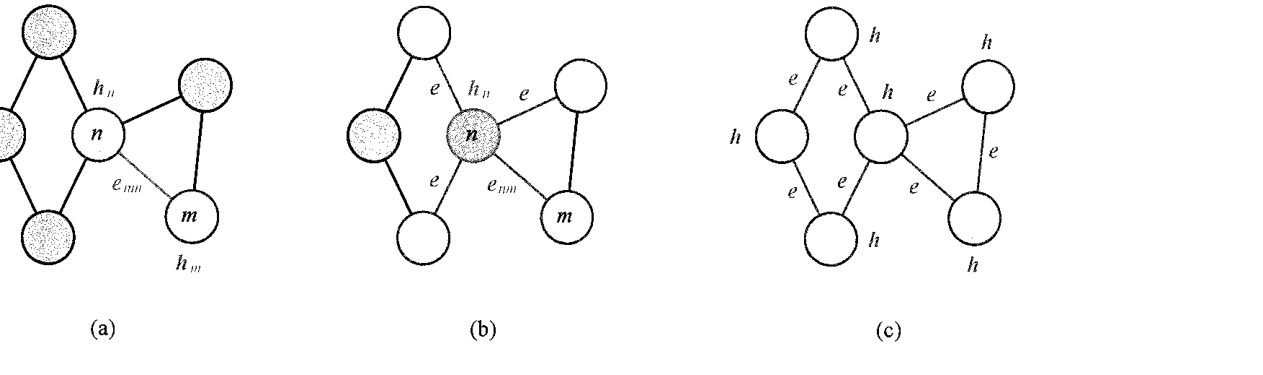
\includegraphics[width=0.9\textwidth]{ch13-fig13.5-msg-update.png}
\caption{式\eqref{align:ch13-edge-update-g}～式\eqref{align:ch13-graph-update}定义的图消息传递更新的示意图，展示了~(a)~边更新、(b)~节点更新，以及~(c)~全局图更新。在每种情况下，正在更新的变量用红色显示，而那些对该更新有贡献的变量则用蓝色显示。}
\label{fig:ch13-msg-update}
\end{figure}

\subsection{过度平滑}\label{subsection:ch13-过度平滑}

某些图神经网络会出现的一个显著问题，就是所谓的过度平滑（over-smoothing），在多次迭代地进行消息传递后，节点嵌入向量变得彼此非常相似，这实际上限制了网络的深度。缓解这个问题的一种方法是引入残差连接（见~9.5~节）。例如，我们可以修改更新运算符[式\eqref{align:ch13-node-update-g}]：
\begin{align}
\bm{h}_n^{(l+1)}=\operatorname{Update}_{\mathrm{node}}\!\left(\bm{h}_n^{(l)},\bm{z}_n^{(l+1)},\bm{g}^{(l)}\right)+\bm{h}_n^{(l)}.
\label{align:ch13-residual}
\end{align}

减少过度平滑的另一种方法是让输出层不仅从网络的最后一个卷积层获取信息，也从所有先前层获取信息。这可以通过拼接先前层的表示来完成：
\begin{align}
\bm{y}_n=f\!\left(\bm{h}_n^{(1)}\oplus\bm{h}_n^{(2)}\oplus\cdots\oplus\bm{h}_n^{(L)}\right)
\label{align:ch13-jump}
\end{align}
其中 $\bm{a}\oplus\bm{b}$ 表示对向量 $\bm{a}$ 和 $\bm{b}$ 进行拼接。这种方法的一个变体是使用最大池化（max pooling）而不是拼接来组合向量。在这种情况下，输出向量的每个元素由前几层中所有对应嵌入向量的元素的最大值决定。

\subsection{正则化}\label{subsection:ch13-正则化}

标准的正则化技术可以用于图神经网络（参见第~9~章），包括将惩罚项（例如参数值的平方和）添加到损失函数中。此外，一些专门针对图神经网络开发的正则化方法也已经出现。

图神经网络已经采用权重共享来实现置换的等变性和不变性，但通常它们在每层都有独立的参数。然而，权重和偏置也可以跨层共享，以减少独立参数的数量。

在图神经网络的背景下进行~dropout~指的是在训练期间省略图节点的随机子集，对于每次前向传播则选择新的随机子集。这同样适用于图中的边，即在训练过程中，随机移除或掩盖邻接矩阵中的部分元素。

\subsection{几何深度学习}\label{subsection:ch13-几何深度学习}

在设计针对图结构数据的深度学习模型时，我们已经看到排列对称性是一个至关重要的因素。它作为一种归纳偏置的形式，在大幅减少数据需求的同时也提高了预测性能。在与空间属性相关的图神经网络应用中，如图形网格、流体流动模拟或分子结构，我们还可以在网络架构中构建额外的等变性和不变性。

例如，考虑预测分子属性的任务。当探索候选药物的空间时，分子可以表示为一个列表，其中包括给定类型的原子（碳原子、氢原子、氮原子等）以及每个原子的空间坐标（表示为三维的列向量）。我们可以为每个原子 $n$ 在每一层 $l$ 引入一个相关的嵌入向量，表示为 $\bm{r}_n^{(l)}$，并且这些向量可以用已知的原子坐标进行初始化。然而，这些向量的元素值取决于坐标系统的任意选择，而分子的属性则不依赖于它。例如，如果分子在三维空间中旋转或相对于坐标系统原点移动到新位置，或者如果坐标系统本身反射得到分子的镜像版本，那么分子的溶解度保持不变。因此，分子的属性也应该在这样的变换下保持不变。

通过仔细选择更新操作和聚合操作的函数形式（Satorras, Hoogeboom, and Welling, 2021），新的嵌入向量 $\bm{r}_n^{(l)}$ 可以纳入图神经网络的更新方程[式\eqref{align:ch13-edge-update}～式\eqref{align:ch13-edge-node-update}]中，以实现所需的对称性：
\begin{align}
\bm{e}_{nm}^{(l+1)}&=\operatorname{Update}_{\mathrm{edge}}\!\left(\bm{e}_{nm}^{(l)},\bm{h}_n^{(l)},\bm{h}_m^{(l)},\|\bm{r}_n^{(l)}-\bm{r}_m^{(l)}\|^2\right)
\label{align:ch13-geo-edge}\\
\bm{r}_n^{(l+1)}&=\bm{r}_n^{(l)}+C\sum_{(n,m)\in\mathcal{E}}\!\left(\bm{r}_n^{(l)}-\bm{r}_m^{(l)}\right)\phi\!\left(\bm{e}_{nm}^{(l+1)}\right)
\label{align:ch13-geo-coord}\\
\bm{z}_n^{(l+1)}&=\operatorname{Aggregate}_{\mathrm{node}}\!\left(\{\bm{e}_{nm}^{(l+1)}:m\in\mathcal{N}(n)\}\right)
\label{align:ch13-geo-agg}\\
\bm{h}_n^{(l+1)}&=\operatorname{Update}_{\mathrm{node}}\!\left(\bm{h}_n^{(l)},\bm{z}_n^{(l+1)}\right).
\label{align:ch13-geo-node}
\end{align}

注意，$\|\bm{r}_n^{(l)}-\bm{r}_m^{(l)}\|^2$ 表示坐标 $\bm{r}_n^{(l)}$ 和 $\bm{r}_m^{(l)}$ 之间的平方距离，它并不依赖于平移、旋转或反射。同样，坐标 $\bm{r}_n^{(l)}$ 可以通过相对差异 $(\bm{r}_n^{(l)}-\bm{r}_m^{(l)})$ 的线性组合进行更新。这里的 $\phi(\bm{e}_{nm}^{(l+1)})$ 是边嵌入的一般标量函数，由神经网络表示，系数 $C$ 通常设置为求和项数目的倒数。因此在这种变换下，消息传递方程[式\eqref{align:ch13-geo-edge}、式\eqref{align:ch13-geo-agg}和式\eqref{align:ch13-geo-node}]是不变的，而式\eqref{align:ch13-geo-coord}给出的坐标嵌入是等变的（见习题~13.10）。

我们已经看到了结构化数据中许多对称性的例子，从图像中物体的平移和图中节点顺序的排列，到三维空间中分子的旋转和平移。将这些对称性捕获在深度神经网络的结构中是一种强大的归纳偏置形式，也是进行丰富的几何深度学习（geometric deep learning）研究的基础（Bronstein et al., 2017; Bronstein et al., 2021）。

\end{document}
